% Options for packages loaded elsewhere
\PassOptionsToPackage{unicode}{hyperref}
\PassOptionsToPackage{hyphens}{url}
%
\documentclass[
]{article}
\usepackage{amsmath,amssymb}
\usepackage{lmodern}
\usepackage{ifxetex,ifluatex}
\ifnum 0\ifxetex 1\fi\ifluatex 1\fi=0 % if pdftex
  \usepackage[T1]{fontenc}
  \usepackage[utf8]{inputenc}
  \usepackage{textcomp} % provide euro and other symbols
\else % if luatex or xetex
  \usepackage{unicode-math}
  \defaultfontfeatures{Scale=MatchLowercase}
  \defaultfontfeatures[\rmfamily]{Ligatures=TeX,Scale=1}
\fi
% Use upquote if available, for straight quotes in verbatim environments
\IfFileExists{upquote.sty}{\usepackage{upquote}}{}
\IfFileExists{microtype.sty}{% use microtype if available
  \usepackage[]{microtype}
  \UseMicrotypeSet[protrusion]{basicmath} % disable protrusion for tt fonts
}{}
\makeatletter
\@ifundefined{KOMAClassName}{% if non-KOMA class
  \IfFileExists{parskip.sty}{%
    \usepackage{parskip}
  }{% else
    \setlength{\parindent}{0pt}
    \setlength{\parskip}{6pt plus 2pt minus 1pt}}
}{% if KOMA class
  \KOMAoptions{parskip=half}}
\makeatother
\usepackage{xcolor}
\IfFileExists{xurl.sty}{\usepackage{xurl}}{} % add URL line breaks if available
\IfFileExists{bookmark.sty}{\usepackage{bookmark}}{\usepackage{hyperref}}
\hypersetup{
  pdftitle={Process data from reproducibility service},
  pdfauthor={Lars Vilhuber},
  hidelinks,
  pdfcreator={LaTeX via pandoc}}
\urlstyle{same} % disable monospaced font for URLs
\usepackage[margin=1in]{geometry}
\usepackage{color}
\usepackage{fancyvrb}
\newcommand{\VerbBar}{|}
\newcommand{\VERB}{\Verb[commandchars=\\\{\}]}
\DefineVerbatimEnvironment{Highlighting}{Verbatim}{commandchars=\\\{\}}
% Add ',fontsize=\small' for more characters per line
\usepackage{framed}
\definecolor{shadecolor}{RGB}{248,248,248}
\newenvironment{Shaded}{\begin{snugshade}}{\end{snugshade}}
\newcommand{\AlertTok}[1]{\textcolor[rgb]{0.94,0.16,0.16}{#1}}
\newcommand{\AnnotationTok}[1]{\textcolor[rgb]{0.56,0.35,0.01}{\textbf{\textit{#1}}}}
\newcommand{\AttributeTok}[1]{\textcolor[rgb]{0.77,0.63,0.00}{#1}}
\newcommand{\BaseNTok}[1]{\textcolor[rgb]{0.00,0.00,0.81}{#1}}
\newcommand{\BuiltInTok}[1]{#1}
\newcommand{\CharTok}[1]{\textcolor[rgb]{0.31,0.60,0.02}{#1}}
\newcommand{\CommentTok}[1]{\textcolor[rgb]{0.56,0.35,0.01}{\textit{#1}}}
\newcommand{\CommentVarTok}[1]{\textcolor[rgb]{0.56,0.35,0.01}{\textbf{\textit{#1}}}}
\newcommand{\ConstantTok}[1]{\textcolor[rgb]{0.00,0.00,0.00}{#1}}
\newcommand{\ControlFlowTok}[1]{\textcolor[rgb]{0.13,0.29,0.53}{\textbf{#1}}}
\newcommand{\DataTypeTok}[1]{\textcolor[rgb]{0.13,0.29,0.53}{#1}}
\newcommand{\DecValTok}[1]{\textcolor[rgb]{0.00,0.00,0.81}{#1}}
\newcommand{\DocumentationTok}[1]{\textcolor[rgb]{0.56,0.35,0.01}{\textbf{\textit{#1}}}}
\newcommand{\ErrorTok}[1]{\textcolor[rgb]{0.64,0.00,0.00}{\textbf{#1}}}
\newcommand{\ExtensionTok}[1]{#1}
\newcommand{\FloatTok}[1]{\textcolor[rgb]{0.00,0.00,0.81}{#1}}
\newcommand{\FunctionTok}[1]{\textcolor[rgb]{0.00,0.00,0.00}{#1}}
\newcommand{\ImportTok}[1]{#1}
\newcommand{\InformationTok}[1]{\textcolor[rgb]{0.56,0.35,0.01}{\textbf{\textit{#1}}}}
\newcommand{\KeywordTok}[1]{\textcolor[rgb]{0.13,0.29,0.53}{\textbf{#1}}}
\newcommand{\NormalTok}[1]{#1}
\newcommand{\OperatorTok}[1]{\textcolor[rgb]{0.81,0.36,0.00}{\textbf{#1}}}
\newcommand{\OtherTok}[1]{\textcolor[rgb]{0.56,0.35,0.01}{#1}}
\newcommand{\PreprocessorTok}[1]{\textcolor[rgb]{0.56,0.35,0.01}{\textit{#1}}}
\newcommand{\RegionMarkerTok}[1]{#1}
\newcommand{\SpecialCharTok}[1]{\textcolor[rgb]{0.00,0.00,0.00}{#1}}
\newcommand{\SpecialStringTok}[1]{\textcolor[rgb]{0.31,0.60,0.02}{#1}}
\newcommand{\StringTok}[1]{\textcolor[rgb]{0.31,0.60,0.02}{#1}}
\newcommand{\VariableTok}[1]{\textcolor[rgb]{0.00,0.00,0.00}{#1}}
\newcommand{\VerbatimStringTok}[1]{\textcolor[rgb]{0.31,0.60,0.02}{#1}}
\newcommand{\WarningTok}[1]{\textcolor[rgb]{0.56,0.35,0.01}{\textbf{\textit{#1}}}}
\usepackage{longtable,booktabs,array}
\usepackage{calc} % for calculating minipage widths
% Correct order of tables after \paragraph or \subparagraph
\usepackage{etoolbox}
\makeatletter
\patchcmd\longtable{\par}{\if@noskipsec\mbox{}\fi\par}{}{}
\makeatother
% Allow footnotes in longtable head/foot
\IfFileExists{footnotehyper.sty}{\usepackage{footnotehyper}}{\usepackage{footnote}}
\makesavenoteenv{longtable}
\usepackage{graphicx}
\makeatletter
\def\maxwidth{\ifdim\Gin@nat@width>\linewidth\linewidth\else\Gin@nat@width\fi}
\def\maxheight{\ifdim\Gin@nat@height>\textheight\textheight\else\Gin@nat@height\fi}
\makeatother
% Scale images if necessary, so that they will not overflow the page
% margins by default, and it is still possible to overwrite the defaults
% using explicit options in \includegraphics[width, height, ...]{}
\setkeys{Gin}{width=\maxwidth,height=\maxheight,keepaspectratio}
% Set default figure placement to htbp
\makeatletter
\def\fps@figure{htbp}
\makeatother
\setlength{\emergencystretch}{3em} % prevent overfull lines
\providecommand{\tightlist}{%
  \setlength{\itemsep}{0pt}\setlength{\parskip}{0pt}}
\setcounter{secnumdepth}{-\maxdimen} % remove section numbering
\ifluatex
  \usepackage{selnolig}  % disable illegal ligatures
\fi

\title{Process data from reproducibility service}
\author{Lars Vilhuber}
\date{2021-03-16}

\begin{document}
\maketitle

{
\setcounter{tocdepth}{2}
\tableofcontents
}
\begin{quote}
Note: The
\href{https://aeadataeditor.github.io/processing-jira-process-data/README.pdf}{PDF
version} of this document is transformed by manually printing from a
browser.
\end{quote}

\hypertarget{citation}{%
\subsection{Citation}\label{citation}}

\begin{quote}
Vilhuber, Lars. 2021. ``Process data for the AEA Pre-publication
Verification Service.'' \emph{American Economic Association
{[}publisher{]}}. Ann Arbor, MI: Inter-university Consortium for
Political and Social Research {[}distributor{]}, 2021-03-16.
\url{https://doi.org/10.3886/E117876V2}
\end{quote}

\begin{verbatim}
@techreport{10.3886/e117876v2,
  doi = {10.3886/E117876V2},
  url = {https://www.openicpsr.org/openicpsr/project/117876/version/V2/view},
  author = {Vilhuber,  Lars},
  title = {Process data for the AEA Pre-publication Verification Service},
  institution = {American Economic Association [publisher]},
  series = {ICPSR - Interuniversity Consortium for Political and Social Research},
  year = {2021}
}
\end{verbatim}

\hypertarget{requirements}{%
\subsection{Requirements}\label{requirements}}

This project requires

\begin{itemize}
\tightlist
\item
  R (last run with R 4.0.5)

  \begin{itemize}
  \tightlist
  \item
    package \texttt{here} (\textgreater=0.1)
  \end{itemize}
\end{itemize}

Other packages might be installed automatically by the programs, as long
as the requirements above are met, see
\protect\hyperlink{r-session-info}{Session Info}.

\hypertarget{data}{%
\subsection{Data}\label{data}}

\hypertarget{the-workflow}{%
\subsubsection{The workflow}\label{the-workflow}}

\begin{figure}
\centering
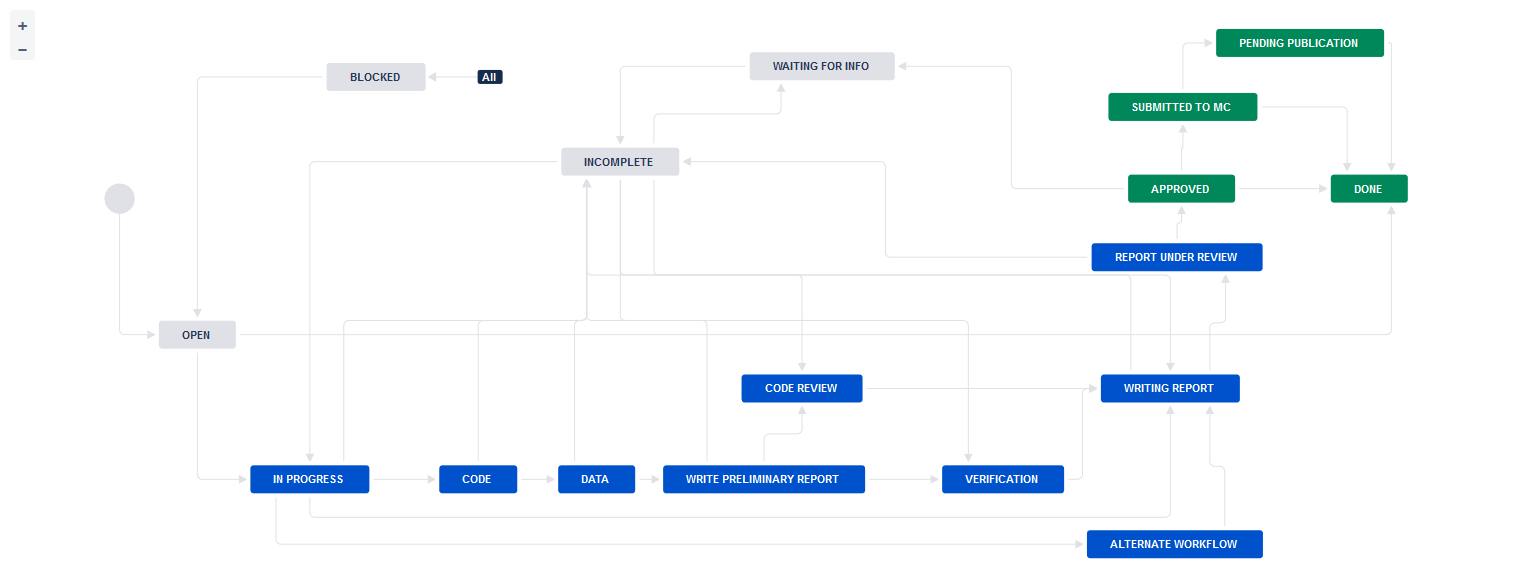
\includegraphics{images/AEADataEditorWorkflow-20191028.png}
\caption{Workflow stages}
\end{figure}

\hypertarget{raw-process-data}{%
\subsubsection{Raw process data}\label{raw-process-data}}

Raw process data is manually extracted from Jira, and saved as

\begin{itemize}
\tightlist
\item
  \texttt{export\_MM-DD-YYYY.csv} (for detailed transaction-level data)
\end{itemize}

The data is not made available outside of the organization, as it
contains names of replicators, manuscript numbers, and verbatim email
correspondence.

At this time, the latest extract was made 05-31-2021.

\hypertarget{anonymized-data}{%
\subsubsection{Anonymized data}\label{anonymized-data}}

We subset the raw data to variables of interest, and substitute random
numbers for sensitive strings. This is done by running
\texttt{01\_jira\_anonymize.R}. The programs saves both the confidential
version and the anonymized version.

\begin{Shaded}
\begin{Highlighting}[]
\FunctionTok{source}\NormalTok{(}\FunctionTok{file.path}\NormalTok{(programs,}\StringTok{"01\_jira\_anonymize.R"}\NormalTok{),}\AttributeTok{echo=}\ConstantTok{TRUE}\NormalTok{)}
\end{Highlighting}
\end{Shaded}

\hypertarget{publishing-data}{%
\subsubsection{Publishing data}\label{publishing-data}}

Some additional cleaning and matching, and then we write out the file

\begin{Shaded}
\begin{Highlighting}[]
\FunctionTok{source}\NormalTok{(}\FunctionTok{file.path}\NormalTok{(programs,}\StringTok{"02\_jira\_anon\_publish.R"}\NormalTok{),}\AttributeTok{echo=}\ConstantTok{TRUE}\NormalTok{)}
\end{Highlighting}
\end{Shaded}

\hypertarget{describing-the-data}{%
\subsection{Describing the Data}\label{describing-the-data}}

The anonymized data has 15 columns.

\hypertarget{variables}{%
\subsubsection{Variables}\label{variables}}

\begin{verbatim}
## 
## -- Column specification --------------------------------------------------------
## cols(
##   name = col_character(),
##   label = col_character()
## )
\end{verbatim}

\begin{longtable}[]{@{}
  >{\raggedright\arraybackslash}p{(\columnwidth - 2\tabcolsep) * \real{0.10}}
  >{\raggedright\arraybackslash}p{(\columnwidth - 2\tabcolsep) * \real{0.90}}@{}}
\toprule
name & label \\
\midrule
\endhead
ticket & The tracking number within the system. Project specific.
Sequentially assigned upon receipt. \\
date\_created & Date of a receipt \\
date\_updated & Date of a transaction \\
mc\_number\_anon & The (anonymized) number assigned by the editorial
workflow system (Manuscript Central/ ScholarOne) to a manuscript. This
is purged by a script of any revision suffixes. \\
Journal & Journal associated with an issue and manuscript. Derived from
the manuscript number. Possibly updated by hand \\
Status & Status associated with a ticket at any point in time. The
schema for these has changed over time. \\
Software.used & A list of software used to replicate the issue. \\
received & An indicator for whether the issue is just created and has
not been assigned to a replicator yet. \\
Changed.Fields & A transaction will change various fields. These are
listed here. \\
external & An indicator for whether the issue required the external
validation. \\
subtask & An indicator for whether the issue is a subtask of another
task. \\
Resolution & Resolution associated with a ticket at the end of the
replication process. \\
reason.failure & A list of reasons for failure to fully replicate. \\
MCRecommendation & Decision status when the issue is Revise and
Resubmit. \\
MCRecommendationV2 & Decision status when the issue is conditionally
accepted. \\
\bottomrule
\end{longtable}

\hypertarget{sample-records}{%
\subsubsection{Sample records}\label{sample-records}}

\begin{longtable}[]{@{}
  >{\raggedright\arraybackslash}p{(\columnwidth - 28\tabcolsep) * \real{0.06}}
  >{\raggedright\arraybackslash}p{(\columnwidth - 28\tabcolsep) * \real{0.06}}
  >{\raggedright\arraybackslash}p{(\columnwidth - 28\tabcolsep) * \real{0.06}}
  >{\raggedleft\arraybackslash}p{(\columnwidth - 28\tabcolsep) * \real{0.07}}
  >{\raggedright\arraybackslash}p{(\columnwidth - 28\tabcolsep) * \real{0.05}}
  >{\raggedright\arraybackslash}p{(\columnwidth - 28\tabcolsep) * \real{0.03}}
  >{\raggedright\arraybackslash}p{(\columnwidth - 28\tabcolsep) * \real{0.07}}
  >{\raggedright\arraybackslash}p{(\columnwidth - 28\tabcolsep) * \real{0.04}}
  >{\raggedright\arraybackslash}p{(\columnwidth - 28\tabcolsep) * \real{0.15}}
  >{\raggedright\arraybackslash}p{(\columnwidth - 28\tabcolsep) * \real{0.04}}
  >{\raggedright\arraybackslash}p{(\columnwidth - 28\tabcolsep) * \real{0.04}}
  >{\raggedright\arraybackslash}p{(\columnwidth - 28\tabcolsep) * \real{0.05}}
  >{\raggedright\arraybackslash}p{(\columnwidth - 28\tabcolsep) * \real{0.07}}
  >{\raggedright\arraybackslash}p{(\columnwidth - 28\tabcolsep) * \real{0.08}}
  >{\raggedright\arraybackslash}p{(\columnwidth - 28\tabcolsep) * \real{0.09}}@{}}
\toprule
ticket & date\_created & date\_updated & mc\_number\_anon & Journal &
Status & Software.used & received & Changed.Fields & external & subtask
& Resolution & reason.failure & MCRecommendation & MCRecommendationV2 \\
\midrule
\endhead
AEAREP-1676 & 2020-12-21 & 2020-12-21 & 481 & AEJ:Micro & Open & & No &
Journal & No & NA & & & & \\
AEAREP-1676 & 2020-12-21 & 2020-12-21 & 481 & & Open & & No & Manuscript
Central identifier & No & NA & & & & \\
AEAREP-1676 & 2020-12-21 & 2020-12-21 & 481 & & Open & & Yes & & No & NA
& & & & \\
AEAREP-1674 & 2020-12-18 & 2020-12-21 & 480 & AER & Open & & No &
openICPSR Project Number & No & NA & & & & \\
AEAREP-1674 & 2020-12-18 & 2020-12-18 & 480 & AER & Open & & No &
Journal & No & NA & & & & \\
AEAREP-1674 & 2020-12-18 & 2020-12-18 & 480 & & Open & & No & Manuscript
Central identifier & No & NA & & & & \\
\bottomrule
\end{longtable}

\hypertarget{r-session-info}{%
\subsubsection{R session info}\label{r-session-info}}

\begin{Shaded}
\begin{Highlighting}[]
\FunctionTok{sessionInfo}\NormalTok{()}
\end{Highlighting}
\end{Shaded}

\begin{verbatim}
## R version 4.0.5 (2021-03-31)
## Platform: x86_64-w64-mingw32/x64 (64-bit)
## Running under: Windows 10 x64 (build 19042)
## 
## Matrix products: default
## 
## locale:
## [1] LC_COLLATE=English_United States.1252 
## [2] LC_CTYPE=English_United States.1252   
## [3] LC_MONETARY=English_United States.1252
## [4] LC_NUMERIC=C                          
## [5] LC_TIME=English_United States.1252    
## 
## attached base packages:
## [1] stats     graphics  grDevices utils     datasets  methods   base     
## 
## other attached packages:
## [1] readr_1.4.0   knitr_1.30    tidyr_1.1.2   stringr_1.4.0 dplyr_1.0.2  
## 
## loaded via a namespace (and not attached):
##  [1] rstudioapi_0.13  magrittr_2.0.1   hms_1.0.0        tidyselect_1.1.0
##  [5] here_1.0.0       R6_2.5.0         rlang_0.4.10     fansi_0.4.2     
##  [9] highr_0.8        tools_4.0.5      xfun_0.22        utf8_1.1.4      
## [13] cli_2.3.1        htmltools_0.5.0  ellipsis_0.3.1   assertthat_0.2.1
## [17] yaml_2.2.1       rprojroot_2.0.2  digest_0.6.27    tibble_3.0.6    
## [21] lifecycle_1.0.0  crayon_1.4.1     purrr_0.3.4      vctrs_0.3.6     
## [25] glue_1.4.2       evaluate_0.14    rmarkdown_2.5    stringi_1.5.3   
## [29] compiler_4.0.5   pillar_1.5.0     generics_0.1.0   pkgconfig_2.0.3
\end{verbatim}

\end{document}
